
\chapter{Demo Chapter}
this is just a demo ref, but it is cool: \cite{kaltenbrunner2018tquencer}

\section*{LaTeX Diagram Demo}

Here is an example of a simple diagram drawn using TikZ:

\begin{center}
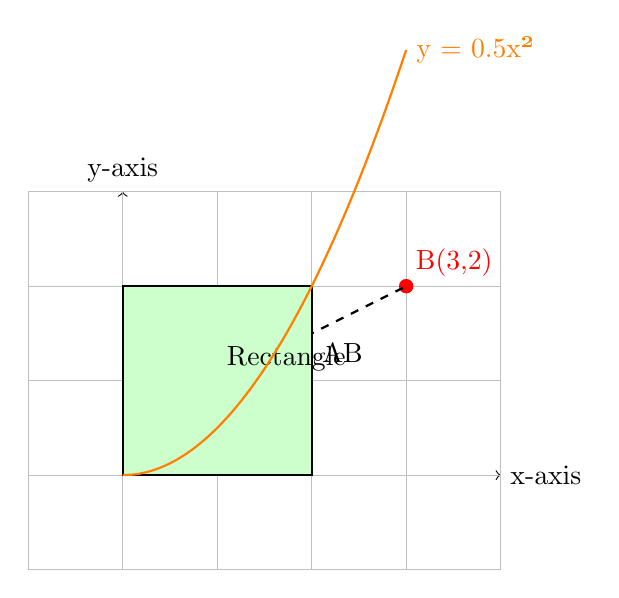
\begin{tikzpicture}[scale=1.2]
    % Draw axes
    \draw[->] (-1, 0) -- (4, 0) node[right] {x-axis};
    \draw[->] (0, -1) -- (0, 3) node[above] {y-axis};
    
    % Add grid lines
    \draw[help lines, step=1cm, gray!50] (-1, -1) grid (4, 3);
    
    % Plot points
    \filldraw[blue] (1, 1) circle (2pt) node[above right] {A(1,1)};
    \filldraw[red] (3, 2) circle (2pt) node[above right] {B(3,2)};
    
    % Draw line connecting points
    \draw[thick, dashed] (1, 1) -- (3, 2) node[midway, below] {Line AB};
    
    % Add a rectangle
    \draw[thick, fill=green!20] (0, 0) rectangle (2, 2);
    \node[above right] at (1, 1) {Rectangle};
    
    % Add a labeled curve
    \draw[domain=0:3, smooth, variable=\x, thick, orange] 
        plot (\x, {0.5*\x*\x}) node[right] {y = 0.5x²};
\end{tikzpicture}
\end{center}

\section*{LaTeX Math Equation Demo}

Here are some examples of math equations in LaTeX:

\subsection*{Inline Math}
The quadratic formula is written as \( x = \frac{-b \pm \sqrt{b^2 - 4ac}}{2a} \).

\subsection*{Displayed Equations}
The same formula in a displayed equation:
\[
x = \frac{-b \pm \sqrt{b^2 - 4ac}}{2a}
\]

\subsection*{Aligned Equations}
Solving a system of linear equations:
\begin{align*}
2x + 3y &= 5 \\
4x -  y &= 7
\end{align*}

\subsection*{Matrices}
A 3x3 identity matrix:
\[
I_3 = 
\begin{bmatrix}
1 & 0 & 0 \\
0 & 1 & 0 \\
0 & 0 & 1
\end{bmatrix}
\]

\subsection*{Summations and Integrals}
A summation example:
\[
S = \sum_{n=1}^\infty \frac{1}{n^2}
\]

An integral example:
\[
\int_a^b x^2 \, dx = \frac{b^3}{3} - \frac{a^3}{3}
\]

\subsection*{Greek Letters and Symbols}
Using Greek letters and mathematical symbols:
\[
\alpha + \beta = \gamma, \quad \nabla \cdot \mathbf{F} = \frac{\partial F_x}{\partial x} + \frac{\partial F_y}{\partial y} + \frac{\partial F_z}{\partial z}
\]
